\documentclass{BeamerTemplate}

\usepackage{pgfplotstable}
\pgfplotsset{compat=1.17}

% Données de l'exemple 1 : production (kg) de 60 plants de tomates
\pgfplotstableread{
x y
3 2.92
3 2.59
3 2.73
3 2.43
3 3.78
3 2.23
3 3.07
3 1.69
3 1.98
3 2.95
4 2.54
4 2.92
4 3.65
4 3.57
4 3.60
4 2.41
4 3.79
4 2.74
4 2.41
4 3.49
5 3.17
5 2.72
5 4.53
5 3.21
5 3.00
5 4.15
5 2.99
5 4.48
5 3.17
5 3.82
6 4.13
6 4.64
6 4.55
6 3.42
6 4.23
6 3.76
6 3.57
6 4.94
6 3.93
6 3.46
7 3.42
7 5.20
7 4.63
7 4.16
7 3.64
7 3.61
7 4.44
7 4.46
7 5.08
7 4.23
8 4.08
8 5.43
8 5.76
8 3.99
8 4.55
8 4.93
8 5.11
8 5.00
8 4.86
8 4.72
}\tomates

% Style du nuage de points des tomates
\pgfplotsset{
  tomates/.style={
    width=9.5cm, height=6cm, xmin=2.6, xmax=8.4, ymin=1.4, ymax=6,
    xlabel={Heures d'ensoleillement}, ylabel={Production (kg)},
    tick label style={font=\scriptsize}, label style={font=\small},
    grid=major, grid style={black!10},
  }
}

\title{Chapitre 6a -- Régression linéaire simple}
\subtitle{STT-1920 Méthodes statistiques}
\date{}

\begin{document}
\begin{frame}[t]
  \titlepage
\end{frame}

\begin{frame}[t]{Plan}
\tableofcontents
\end{frame}

%-------------------------------------------------------------------------------
\section{Introduction}
%-------------------------------------------------------------------------------

\begin{frame}[t]{Objectifs de la régression linéaire simple}

\begin{itemize}\itemsep3mm
  \item Vérifier si une \alert{relation linéaire} existe entre les variables
  aléatoires $X$ (variable \alert{explicative}) et $Y$ (variable \alert{réponse}).
  \item<2-> Mesurer la \alert{force} du lien linéaire qui unit les variables.
  \item<3-> Trouver la \alert{meilleure droite} exprimant la relation entre les
  deux variables à partir de $n$ paires d'observations indépendantes $(X_i,Y_i)$.
  Évaluer la précision des estimations de la pente et de l'ordonnée à l'origine.
  \item<4-> \alert{Prédire} la valeur de $Y$ pour un $X$ donné, et évaluer la
  précision de ces prédictions.
\end{itemize}

\end{frame}

\begin{frame}[t]{Trois grands usages de la régression}

\begin{itemize}\itemsep4mm
  \item \alert{Décrire}: quelle est la forme et la force du lien entre deux
  variables?\\
  {\small Ex.: comment l'envergure d'une hirondelle varie-t-elle avec son poids?}
  \item<2-> \alert{Prédire}: quelle valeur de $Y$ peut-on attendre pour une valeur
  de $X$ donnée?\\
  {\small Ex.: quelle production attendre d'un plant de tomates qui reçoit 6,5\,h de
  soleil par jour?}
  \item<3-> \alert{Contrôler}: quelle valeur de $X$ faut-il fixer pour obtenir, en
  moyenne, la valeur de $Y$ désirée?\\
  {\small Ex.: combien d'heures d'ensoleillement faut-il fournir pour qu'un plant
  produise en moyenne 4\,kg de tomates?}
\end{itemize}

\end{frame}

\begin{frame}[t]{Exemples d'application}

\begin{itemize}\itemsep2mm
  \item Un sociologue veut savoir s'il existe un lien linéaire entre le nombre
  d'années d'études et le salaire à l'embauche.
  \item<2-> Un médecin veut étudier la relation entre l'IMC des individus et le taux
  de cholestérol dans leur sang.
  \item<3-> Un ingénieur veut savoir si le taux d'humidité dans le papier est
  directement proportionnel à la température du séchoir.
  \item<4-> Un économiste veut savoir si le lien entre l'offre d'un produit et son
  prix est linéaire.
  \item<5-> Une écologiste veut savoir si la biomasse d'algues d'un lac augmente
  linéairement avec la concentration de phosphore dans l'eau.
  \item<6-> Une pharmacologue veut relier la dose d'un antihypertenseur à la baisse
  de pression artérielle observée chez les patients.
\end{itemize}

\end{frame}

\begin{frame}[t]{Exemple 1: ensoleillement et production de tomates}

On veut étudier l'effet du nombre d'heures d'\alert{ensoleillement} quotidien sur
la \alert{production} (kg) de tomates. Dans une serre, on contrôle la quantité de
soleil reçue par 60 plants: 10 plants pour chacune des durées 3, 4, 5, 6, 7 et
8 heures par jour. Quatre mois plus tard, on note la production de chaque plant.

\medskip
\begin{center}
\scriptsize
\begin{tabular}{c|cccccccccc}
\toprule
Soleil & \multicolumn{10}{c}{Production (kg)}\\
\midrule
3 h & 2,92 & 2,59 & 2,73 & 2,43 & 3,78 & 2,23 & 3,07 & 1,69 & 1,98 & 2,95\\
4 h & 2,54 & 2,92 & 3,65 & 3,57 & 3,60 & 2,41 & 3,79 & 2,74 & 2,41 & 3,49\\
5 h & 3,17 & 2,72 & 4,53 & 3,21 & 3,00 & 4,15 & 2,99 & 4,48 & 3,17 & 3,82\\
6 h & 4,13 & 4,64 & 4,55 & 3,42 & 4,23 & 3,76 & 3,57 & 4,94 & 3,93 & 3,46\\
7 h & 3,42 & 5,20 & 4,63 & 4,16 & 3,64 & 3,61 & 4,44 & 4,46 & 5,08 & 4,23\\
8 h & 4,08 & 5,43 & 5,76 & 3,99 & 4,55 & 4,93 & 5,11 & 5,00 & 4,86 & 4,72\\
\bottomrule
\end{tabular}
\end{center}

\end{frame}

\begin{frame}[t]{Exemple 1: les 60 plants de tomates}

\begin{center}
\begin{tikzpicture}
\begin{axis}[tomates]
  \addplot[only marks, mark=o, mark size=1.8pt] table[x=x, y=y] {\tomates};
\end{axis}
\end{tikzpicture}
\end{center}

\uncover<2->{La relation entre les deux variables semble \alert{linéaire}.}

\end{frame}

\begin{frame}[t]{Exemple 2: poids et envergure des hirondelles}

On cherche à démontrer qu'il existe un lien linéaire entre le \alert{poids}
d'une hirondelle ($X$, en g) et l'\alert{étendue de ses ailes} ouvertes ($Y$, en cm).
Pour ce faire, on mesure ces deux quantités sur 50 hirondelles choisies au
hasard dans la population d'intérêt.

\medskip
\begin{center}
\scriptsize
\begin{tabular}{ccc}
\toprule
Oiseau & Poids & Étendue\\
\midrule
1 & 52,29 & 14,10\\
2 & 39,05 & 8,94\\
3 & 40,23 & 8,79\\
4 & 43,69 & 9,59\\
5 & 50,23 & 10,60\\
$\vdots$ & $\vdots$ & $\vdots$\\
\bottomrule
\end{tabular}
\hspace{1cm}
\begin{tabular}{ccc}
\toprule
Oiseau & Poids & Étendue\\
\midrule
26 & 48,93 & 12,05\\
27 & 48,17 & 11,13\\
28 & 55,53 & 13,79\\
29 & 50,85 & 13,26\\
30 & 42,88 & 9,51\\
$\vdots$ & $\vdots$ & $\vdots$\\
\bottomrule
\end{tabular}
\end{center}

\end{frame}

% NOTE : les oiseaux 16 à 21 et 41 à 46 étaient illisibles dans les anciennes
% diapos; le nuage ci-dessous ne contient que les 38 autres oiseaux.
% Ajouter les 12 points manquants si les données complètes sont disponibles.
\begin{frame}[t]{Exemple 2: les hirondelles}

\begin{center}
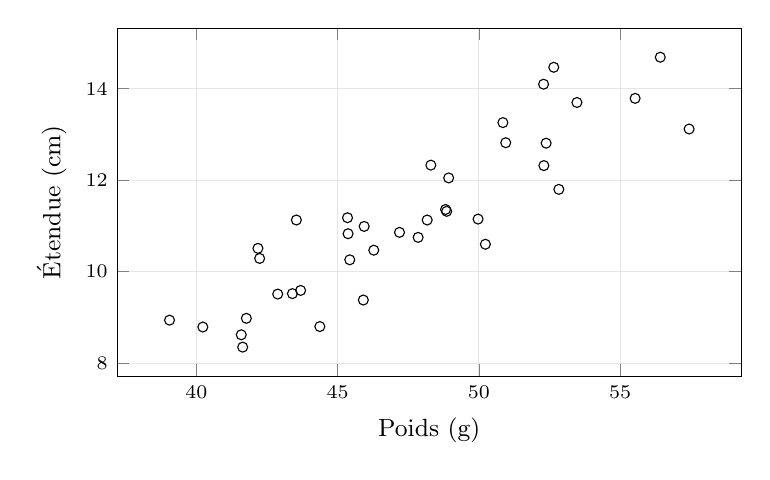
\begin{tikzpicture}
\begin{axis}[width=9.5cm, height=6cm, xlabel={Poids (g)}, ylabel={Étendue (cm)},
  tick label style={font=\scriptsize}, label style={font=\small},
  grid=major, grid style={black!10}]
  \addplot[only marks, mark=o, mark size=1.8pt] coordinates {
  (52.29,14.10) (39.05,8.94) (40.23,8.79) (43.69,9.59) (50.23,10.60)
  (57.44,13.12) (42.18,10.51) (43.54,11.13) (41.59,8.62) (52.38,12.81)
  (45.35,11.18) (52.30,12.32) (45.91,9.38) (47.19,10.86) (45.94,10.99)
  (47.85,10.75) (48.82,11.36) (44.37,8.80) (46.28,10.47)
  (48.93,12.05) (48.17,11.13) (55.53,13.79) (50.85,13.26) (42.88,9.51)
  (48.86,11.32) (52.65,14.47) (45.43,10.26) (43.40,9.52) (50.95,12.82)
  (42.24,10.29) (48.30,12.33) (56.42,14.69) (49.97,11.15) (41.64,8.35)
  (52.83,11.80) (41.77,8.98) (53.47,13.70) (45.37,10.83)};
\end{axis}
\end{tikzpicture}
\end{center}

\end{frame}

\begin{frame}[t]{Attention: association n'est pas causalité!}

\small
\begin{itemize}\itemsep1mm
  \item<1-> \textbf{Tomates} (\alert{expérience contrôlée}): on fixe
  l'ensoleillement. Si les plants sont répartis au hasard entre les durées, on peut
  attribuer à l'ensoleillement les différences de production.
  \item<2-> \textbf{Hirondelles} (\alert{étude observationnelle}): les oiseaux lourds
  ont de plus grandes ailes, mais engraisser une hirondelle n'allongera pas ses
  ailes! Les deux variables dépendent de la taille de l'oiseau.
  \item<3-> Villes: plus de pharmacies $\leftrightarrow$ plus de cas de grippe,
  car les deux augmentent avec la population (\alert{variable confondante}).
\end{itemize}

\uncover<4->{
\begin{Boite}{À retenir}
\small
Un lien, même très fort, \alert{ne prouve pas} que $X$ cause $Y$. Seule une
expérience contrôlée (répartition aléatoire) permet de conclure à un effet causal.
\end{Boite}}

\end{frame}

%-------------------------------------------------------------------------------
\section{Modèle de régression linéaire simple}
%-------------------------------------------------------------------------------

\begin{frame}[t]{Le modèle}

On suppose que $X$ et $Y$ sont reliées par la droite $Y=\beta_0+\beta_1X$, et que
les observations dévient un peu de ce modèle par une erreur aléatoire
$\varepsilon$:

\begin{Boite}{Modèle de régression linéaire simple}
\[
Y_i=\beta_0+\beta_1X_i+\varepsilon_i,\qquad i=1,\ldots,n
\]
\end{Boite}

\begin{itemize}\itemsep1mm
  \item $Y_i$ = $i$\textsuperscript{e} mesure de la variable $Y$;
  \item $X_i$ = $i$\textsuperscript{e} mesure de la variable $X$;
  \item $\beta_0$ =
  \item $\beta_1$ =
  \item $\varepsilon_i$ = perturbation due au hasard ou à des variables autres que
  $X$ (erreur du modèle, différence entre $Y_i$ et la droite).
\end{itemize}

\end{frame}

\begin{frame}[t]{Les postulats}

\begin{itemize}\itemsep1.5mm
  \item[(P1)] \alert{Linéarité}: les variables $X$ et $Y$ sont associées par un
  lien linéaire, i.e.\ $E(Y_i)=\beta_0+\beta_1X_i$.
  \item<2->[(P2)] \alert{Homoscédasticité}: la \alert{variance} des $Y_i$ autour de
  la droite (notée $\sigma^2$) est \alert{constante} pour toutes les valeurs de $X$.
  \item<3->[(P3)] \alert{Indépendance}: les observations $(X_i,Y_i)$ sont
  indépendantes les unes des autres.
  \item<4->[(P4)] \alert{Normalité}: les observations $Y_i$ sont issues d'une loi
  normale pour chaque $X_i$ fixé.
\end{itemize}

\uncover<5->{
\begin{Boite}{En résumé}
$\varepsilon_1,\ldots,\varepsilon_n$ sont indépendantes et de loi $N(0,\sigma^2)$.
\end{Boite}

{\small Ces postulats seront vérifiés au chapitre 6b, à l'aide des résidus.}}

\end{frame}

\begin{frame}[t]{Illustration du modèle}

\begin{center}
\begin{tikzpicture}
\begin{axis}[tomates, height=6cm, ymin=0.9, ymax=6.3]
  \addplot[only marks, mark=o, mark size=1.5pt, black!35] table[x=x, y=y] {\tomates};
  \addplot[burntorange, very thick, domain=2.6:8.4] {1.37242+0.43126*x};
  \addplot[Dominante!70!black, thick, domain=-2.8:2.8, samples=60]
    ({3+0.55*exp(-x^2/2)}, {1.37242+0.43126*3+0.568*x});
  \addplot[Dominante!70!black, dotted] coordinates {(3,1.076) (3,4.257)};
  \addplot[Dominante!70!black, thick, domain=-2.8:2.8, samples=60]
    ({5+0.55*exp(-x^2/2)}, {1.37242+0.43126*5+0.568*x});
  \addplot[Dominante!70!black, dotted] coordinates {(5,1.938) (5,5.119)};
  \addplot[Dominante!70!black, thick, domain=-2.8:2.8, samples=60]
    ({7+0.55*exp(-x^2/2)}, {1.37242+0.43126*7+0.568*x});
  \addplot[Dominante!70!black, dotted] coordinates {(7,2.801) (7,5.982)};
  \node[burntorange, font=\small, anchor=west, fill=white, inner sep=1pt]
    at (axis cs:2.8,5.8) {$E(Y)=\beta_0+\beta_1x$};
\end{axis}
\end{tikzpicture}
\end{center}

{\small Pour chaque $x$ fixé, $Y$ suit une loi normale centrée sur la droite, avec
la même variance $\sigma^2$ (P2 et P4).}

\end{frame}

%-------------------------------------------------------------------------------
\section{Estimation des paramètres}
%-------------------------------------------------------------------------------

\begin{frame}[t]{Estimation par les moindres carrés}

Pour estimer $\beta_0$ et $\beta_1$, on minimise la \alert{somme des carrés des
erreurs}, i.e.\ des écarts verticaux entre les observations $Y_i$ et le point
correspondant sur la droite $\beta_0+\beta_1X_i$:
\[
\sum_{i=1}^{n}\varepsilon_i^2=\sum_{i=1}^{n}\bigl(Y_i-[\beta_0+\beta_1X_i]\bigr)^2.
\]

\uncover<2->{Il suffit donc de dériver cette expression successivement par rapport
à $\beta_0$ et $\beta_1$, d'égaler les dérivées partielles à 0 et de résoudre le
système obtenu pour trouver $\hat\beta_0=b_0$ et $\hat\beta_1=b_1$.}

\end{frame}

\begin{frame}[t]{Estimateurs $b_0$ et $b_1$}

\begin{Boite}{Estimateurs des moindres carrés}
\[
b_1=\frac{\sum_{i=1}^{n}(x_i-\overline{x})(y_i-\overline{y})}
{\sum_{i=1}^{n}(x_i-\overline{x})^2}=\frac{S_{XY}}{S_{XX}},
\qquad
b_0=\overline{y}-b_1\overline{x}.
\]
\end{Boite}

\medskip
La valeur de $Y$ prédite par le modèle pour une valeur de $X$ fixée est donc
\[
\hat y_i=b_0+b_1x_i.
\]

\end{frame}

\begin{frame}[t]{Notations}

\vspace{5mm}
\begin{align*}
S_{XX}&=\sum_{i=1}^{n}(X_i-\overline{X})^2=(n-1)s_X^2\\[3mm]
S_{YY}&=\sum_{i=1}^{n}(Y_i-\overline{Y})^2=(n-1)s_Y^2\\[3mm]
S_{XY}&=\sum_{i=1}^{n}(X_i-\overline{X})(Y_i-\overline{Y})
\end{align*}

\end{frame}

\begin{frame}[t]{Inférence sur les paramètres: distribution de $b_0$ et $b_1$}

$b_0$ et $b_1$ sont des \alert{variables aléatoires}: si on change d'échantillon
$(X_i,Y_i)$, leurs valeurs changent.

\begin{thm}
On peut montrer que
\[
E(b_0)=\beta_0,\qquad E(b_1)=\beta_1,
\]
\[
V(b_0)=\sigma^2\left(\frac1n+\frac{\overline{x}^{\,2}}{S_{XX}}\right),\qquad
V(b_1)=\frac{\sigma^2}{S_{XX}},
\]
et $b_0$ et $b_1$ suivent chacun une loi normale.
\end{thm}

Comme on connaît leur distribution, on peut construire des intervalles de
confiance et des tests.

\end{frame}

\begin{frame}[t]{Remarques}

\begin{itemize}\itemsep1.5cm
  \item
  \item
  \item
  \item
\end{itemize}

\end{frame}

\begin{frame}[fragile,t]{En R: \textsf{Statistiques} $\rightarrow$ \textsf{Ajustement de modèle}}

\begin{Verbatim}[fontsize=\scriptsize]
> RegModel.1 <- lm(production ~ hrs_soleil, data=tomates)
> summary(RegModel.1)

Residuals:
     Min       1Q   Median       3Q      Max
-0.97619 -0.45213  0.00378  0.42100  1.11381

Coefficients:
            Estimate Std. Error t value Pr(>|t|)
(Intercept)  1.37242    0.24733   5.549 7.46e-07 ***
hrs_soleil   0.43126    0.04295  10.042 2.66e-14 ***
---
Signif. codes:  0 '***' 0.001 '**' 0.01 '*' 0.05 '.' 0.1 ' ' 1

Residual standard error: 0.5681 on 58 degrees of freedom
Multiple R-squared:  0.6348,    Adjusted R-squared:  0.6285
F-statistic: 100.8 on 1 and 58 DF,  p-value: 2.661e-14
\end{Verbatim}

\end{frame}

\begin{frame}[fragile,t]{Estimation des paramètres}

\begin{Verbatim}[fontsize=\scriptsize]
            Estimate Std. Error t value Pr(>|t|)
(Intercept)  1.37242    0.24733   5.549 7.46e-07 ***
hrs_soleil   0.43126    0.04295  10.042 2.66e-14 ***
\end{Verbatim}

\begin{columns}[T]
\begin{column}{0.4\textwidth}
\vspace{5mm}
Trouvez et interprétez les estimations des paramètres.
\end{column}
\begin{column}{0.58\textwidth}
\begin{tikzpicture}
\begin{axis}[tomates, width=7.5cm, height=5cm]
  \addplot[only marks, mark=o, mark size=1.5pt] table[x=x, y=y] {\tomates};
  \addplot[burntorange, very thick, domain=2.6:8.4] {1.37242+0.43126*x};
\end{axis}
\end{tikzpicture}
\end{column}
\end{columns}

\end{frame}

\begin{frame}[t]{Interprétation des paramètres $\beta_0$ et $\beta_1$}

\begin{Boite}{Si le postulat de linéarité (P1) est vrai}
\small
\begin{itemize}\itemsep1mm
  \item $\beta_1$: si $X$ augmente d'\alert{une unité}, la \alert{valeur moyenne}
  de $Y$ augmente de $\beta_1$ unités.
  \item $\beta_1>0$: lien positif (grands $X$ associés aux grands $Y$);
  $\beta_1<0$: lien négatif; $\beta_1=0$: aucun lien linéaire.
  \item $\beta_0$: valeur moyenne de $Y$ lorsque $X=0$.
\end{itemize}
\end{Boite}

\small
\begin{itemize}\itemsep1mm
  \item<2-> \textbf{Tomates}: $b_1=0{,}431$\,kg/h. Chaque heure supplémentaire
  d'ensoleillement quotidien augmente la production \alert{moyenne} d'un plant
  d'environ 0,43\,kg (431\,g).
  \item<3-> $b_0=1{,}37$\,kg serait la production moyenne d'un plant sans
  \alert{aucun} soleil\ldots{} Or $x=0$ est loin des durées observées (3 à 8\,h):
  $b_0$ n'a pas d'interprétation réaliste ici. Le modèle reste toutefois utile pour
  des $x$ \alert{proches de ceux observés}.
\end{itemize}

\end{frame}

\begin{frame}[t]{Extrapolation dangereuse!}

\alert{Attention!} On ignore la forme de la relation entre $X$ et $Y$
\alert{à l'extérieur} de l'intervalle des valeurs de $X$ observées.

\begin{columns}[T]
\begin{column}{0.5\textwidth}
\centering
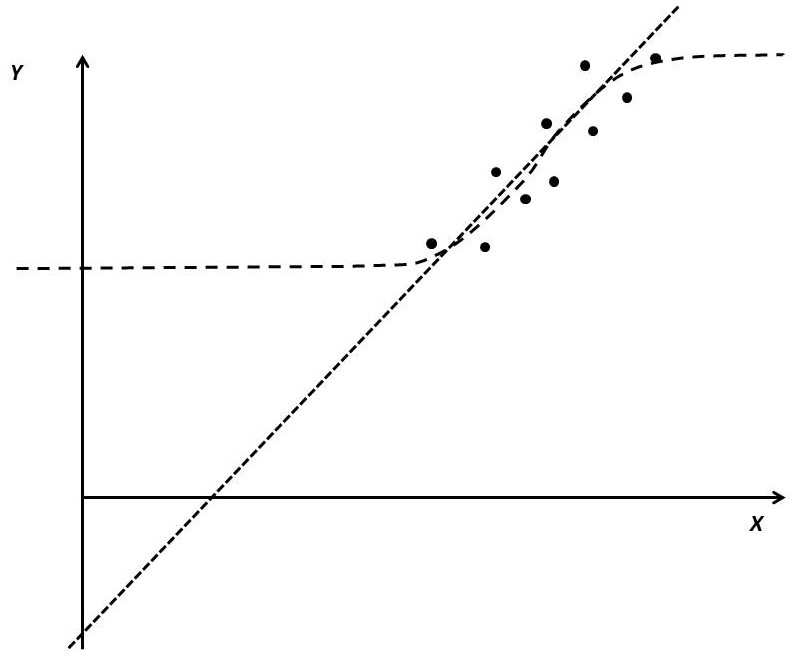
\includegraphics[height=4.4cm]{images/extrapol.jpg}
\end{column}
\begin{column}{0.48\textwidth}
\footnotesize
\begin{itemize}\itemsep2mm
  \item<2-> La vraie relation (courbe pointillée) peut être linéaire là où on a
  des données\ldots{} et tout autre chose ailleurs.
  \item<2-> Tomates: le modèle prédit 1,37\,kg avec 0\,h de soleil et
  $1{,}372+0{,}431\times24=11{,}7$\,kg avec 24\,h par jour. Rien dans les données
  ne permet d'y croire!
  \item<2-> En biologie, les réponses \alert{plafonnent} souvent (saturation,
  toxicité).
\end{itemize}
\end{column}
\end{columns}

\end{frame}

\begin{frame}[plain,t]
  \centerline{\LARGE\bfseries\alert{QUIZ !}}

  \medskip
  Exemple 1 (tomates): $\hat y=1{,}372+0{,}431\,x$.
  \begin{itemize}\itemsep 7mm
    \item Le plant A reçoit 2\,h de soleil de plus par jour que le plant B. Quelle
    différence de production moyenne le modèle prédit-il entre les deux?
    \item<2-> Vrai ou faux: comme $b_1=0{,}43$ est proche de 0, le lien entre
    l'ensoleillement et la production est faible.
    \item<3-> Vrai ou faux: un plant cultivé à l'obscurité totale produit en
    moyenne 1,37\,kg de tomates.
    \item<4-> Combien d'heures de soleil faut-il fournir pour qu'un plant produise
    en moyenne 4\,kg? (usage «\,contrôler\,»)
  \end{itemize}
\end{frame}

% Sortie obtenue en ajustant le modèle aux 38 oiseaux du nuage de points
% (les données des oiseaux 16 à 21 et 41 à 46 sont manquantes).
\begin{frame}[plain,t,fragile]
  \centerline{\LARGE\bfseries\alert{QUIZ !}}

  \medskip
  Exemple 2 (hirondelles): régression de l'étendue des ailes (cm) sur le poids (g).
\begin{Verbatim}[fontsize=\scriptsize]
            Estimate Std. Error t value Pr(>|t|)
(Intercept) -4.42971    1.34034  -3.305  0.00216 **
poids        0.32824    0.02806  11.697 8.05e-14 ***
\end{Verbatim}
  \begin{itemize}\itemsep 1cm
    \item Écrivez l'équation de la droite estimée. Le lien est-il positif ou négatif?
    \item<2-> Interprétez $b_1$ dans le contexte.
    \item<3-> Interprétez $b_0$. A-t-il un sens biologique?
  \end{itemize}
\end{frame}

\begin{frame}[fragile,t]{Intervalles de confiance sur les paramètres}

\begin{Verbatim}[fontsize=\scriptsize]
            Estimate Std. Error t value Pr(>|t|)
(Intercept)  1.37242    0.24733   5.549 7.46e-07 ***
hrs_soleil   0.43126    0.04295  10.042 2.66e-14 ***
\end{Verbatim}

\begin{Boite}{Intervalles de confiance à $(1-\alpha)100\,\%$}
\[
b_1\pm t_{n-2;\,\alpha/2}\sqrt{\frac{MSE}{S_{XX}}},\qquad
b_0\pm t_{n-2;\,\alpha/2}\sqrt{MSE\left(\frac1n+\frac{\overline{x}^{\,2}}{S_{XX}}\right)}
\]
\end{Boite}
{\small où $MSE=SSE/(n-2)$ estime $\sigma^2$ (voir la table d'ANOVA plus loin).}


Calculez un intervalle de confiance à 95\,\% sur la pente et sur l'ordonnée à
l'origine.

\end{frame}

\begin{frame}[fragile,t]{En R: \textsf{Modèles} $\rightarrow$ \textsf{Intervalles de confiance}}

\begin{Verbatim}[fontsize=\small]
> Confint(RegModel.1, level=0.95)
             Estimate     2.5 %    97.5 %
(Intercept) 1.3724190 0.8773266 1.8675115
hrs_soleil  0.4312571 0.3452894 0.5172249
\end{Verbatim}

\bigskip
La relation linéaire entre les heures d'ensoleillement et la production
est-elle significative, au seuil de 5\,\%?
\vspace{2cm}

\end{frame}

\begin{frame}[t]{Interpréter l'intervalle de confiance sur la pente}

\small
Calcul à la main ($t_{58;\,0{,}025}=2{,}0017$; l'erreur-type
$\sqrt{MSE/S_{XX}}=0{,}04295$ est la colonne \texttt{Std.\ Error}):
\[
0{,}43126\pm2{,}0017\times0{,}04295=0{,}43126\pm0{,}08597
\quad\Rightarrow\quad[0{,}345;\ 0{,}517].
\]

\normalsize
\uncover<2->{
\begin{Boite}{En mots}
Avec 95\,\% de confiance, chaque heure supplémentaire d'ensoleillement quotidien
fait augmenter la production \alert{moyenne} d'un plant de \alert{0,35 à 0,52\,kg}.
\end{Boite}}

\begin{itemize}\itemsep2mm
  \item<3-> L'IC donne un ordre de grandeur de l'effet, pas seulement «\,il y a un
  effet\,».
  \item<3-> Comme 0 n'appartient pas à l'IC, on conclut (au seuil de 5\,\%) que
  $\beta_1\ne0$: la relation linéaire est significative.
  \item<3-> Attention: l'IC porte sur $\beta_1$ (la pente de la population), pas sur
  la production d'un plant en particulier (voir chapitre 6b).
\end{itemize}

\end{frame}

%-------------------------------------------------------------------------------
\section{Test $t$ sur la pente}
%-------------------------------------------------------------------------------

\begin{frame}[t]{Test de Student sur la pente}

La question principale: \alert{existe-t-il un lien linéaire} entre $X$ et $Y$?
On teste $H_0:\beta_1=0$ (aucun lien linéaire) contre $H_1:\beta_1\neq0$.

\uncover<2->{
\begin{Boite}{Statistique du test}
Puisque $b_1\sim N(\beta_1,\ \sigma^2/S_{XX})$, on a, sous $H_0$,
\vspace{-1mm}
\[
T=\frac{b_1-0}{\sqrt{MSE/S_{XX}}}\sim t_{n-2}.
\]
\vspace{-5mm}

\noindent{\footnotesize Même logique qu'au chapitre 3:
(estimation $-$ valeur sous $H_0$)\,/\,erreur-type.}
\end{Boite}}

\uncover<3->{
\centering
\footnotesize
\begin{tabular}{ll@{\hspace{1cm}}ll}
\toprule
$H_1$ & Rejeter $H_0$ si\ldots & $H_1$ & Rejeter $H_0$ si\ldots\\
\midrule
$\beta_1\neq0$ & $|t_{obs}|>t_{n-2;\,\alpha/2}$ & $\beta_1>0$ & $t_{obs}>t_{n-2;\,\alpha}$\\
& & $\beta_1<0$ & $t_{obs}<-t_{n-2;\,\alpha}$\\
\bottomrule
\end{tabular}\par}

\end{frame}

\begin{frame}[fragile,t]{Exemple 1 (suite): la pente est-elle nulle?}

\begin{Verbatim}[fontsize=\scriptsize]
            Estimate Std. Error t value Pr(>|t|)
(Intercept)  1.37242    0.24733   5.549 7.46e-07 ***
hrs_soleil   0.43126    0.04295  10.042 2.66e-14 ***
\end{Verbatim}

\begin{itemize}\itemsep2.5mm
  \item<2-> Statistique observée: $t_{obs}=\dfrac{0{,}43126}{0{,}04295}=10{,}04$
  (colonne \texttt{t value}).
  \item<2-> Valeur critique: $t_{58;\,0{,}025}=2{,}00$. Comme $|t_{obs}|=10{,}04>2{,}00$,
  on \alert{rejette} $H_0$.
  \item<3-> Valeur-p $=P(|T|>10{,}04)=2{,}66\times10^{-14}$ (colonne
  \texttt{Pr(>|t|)}): même conclusion.
  \item<4-> \alert{Conclusion}: au seuil de 5\,\%, il existe un lien linéaire
  significatif entre l'ensoleillement et la production de tomates; la production
  moyenne \alert{augmente} avec l'ensoleillement.
  \item<4-> La ligne \texttt{(Intercept)} teste $H_0:\beta_0=0$, ce qui est rarement
  d'intérêt (ici, $x=0$ n'a même pas de sens).
\end{itemize}

\end{frame}

\begin{frame}[plain,t,fragile]
  \centerline{\LARGE\bfseries\alert{QUIZ !}}

  \medskip
  Exemple 2 (hirondelles), $n=38$:
\begin{Verbatim}[fontsize=\scriptsize]
            Estimate Std. Error t value Pr(>|t|)
(Intercept) -4.42971    1.34034  -3.305  0.00216 **
poids        0.32824    0.02806  11.697 8.05e-14 ***
\end{Verbatim}
  \begin{itemize}\itemsep 7mm
    \item Donnez la statistique et la valeur-p du test de $H_0:\beta_1=0$ contre
    $H_1:\beta_1\neq0$. Que conclut-on au seuil de 5\,\%?
    \item<2-> Calculez un IC à 95\,\% pour $\beta_1$ ($t_{36;\,0{,}025}=2{,}028$) et
    interprétez-le en mots.
    \item<3-> Une ornithologue affirme que l'étendue des ailes augmente en moyenne
    de 0,5\,cm par gramme. Les données la contredisent-elles?
  \end{itemize}
\end{frame}

%-------------------------------------------------------------------------------
\section{Test de Fisher pour la régression}
%-------------------------------------------------------------------------------

\begin{frame}[t]{Hypothèses à tester}

Faire le test de la régression, c'est vérifier si la relation linéaire est
\alert{significative}. Bref, on veut savoir si la pente est nulle ou non.

\medskip
\begin{align*}
H_0&:\\
H_1&:
\end{align*}

\medskip
On sait déjà vérifier si 0 est dans l'intervalle de confiance, et on sait
interpréter le test de Student sur la pente. En mettant cette statistique au
carré, on obtient un \alert{test de Fisher} basé sur la décomposition de la
variabilité des $Y_i$.

\end{frame}

\begin{frame}[t]{Décomposition de la variance}

La variabilité totale dans les données (notée $SST$) peut être décomposée en
deux sources:

\medskip
\begin{itemize}\itemsep3mm
  \item<2-> $SSR$: somme des carrés de la \alert{régression};\\
  variabilité entre les valeurs prédites par le modèle linéaire, i.e.\ la
  variabilité \alert{expliquée par $X$};
  \item<3-> $SSE$: somme des carrés des \alert{erreurs};\\
  variabilité des données autour de la droite pour un $x_i$ donné (source autre
  que $X$, que l'on associe à l'erreur échantillonnale non expliquée par le
  modèle).
\end{itemize}

\uncover<4->{\small Rappel (chapitre 5a): c'est la même idée qu'en ANOVA, où
$SST=SST_R+SSE$.}

\end{frame}

\begin{frame}[t]{Décomposition de la variance: illustration}

\begin{center}
\begin{tikzpicture}
\begin{axis}[tomates, width=10cm, height=6.3cm]
  \addplot[only marks, mark=o, mark size=1.5pt, black!40] table[x=x, y=y] {\tomates};
  \addplot[burntorange, very thick, domain=2.6:8.4] {1.37242+0.43126*x};
  \addplot[Dominante!80!black, thick, dashed, domain=2.6:8.4] {3.74433};
  \node[font=\scriptsize, anchor=west, Dominante!80!black] at (axis cs:2.65,3.9) {$\overline{y}$};
  % Un point pour illustrer les écarts
  \addplot[only marks, mark=*, mark size=2pt] coordinates {(8,5.76)};
  \draw[thick, <->, black!70!green] (axis cs:8.12,3.74433) -- node[right, font=\tiny] {$y_i-\overline{y}$} (axis cs:8.12,5.76);
  \draw[thick, <->, red] (axis cs:7.85,4.82250) -- node[left, font=\tiny] {$y_i-\hat y_i$} (axis cs:7.85,5.76);
  \draw[thick, <->, blue] (axis cs:7.7,3.74433) -- node[left, font=\tiny] {$\hat y_i-\overline{y}$} (axis cs:7.7,4.82250);
\end{axis}
\end{tikzpicture}
\end{center}

\end{frame}

\begin{frame}[t]{Décomposition de la variance}

\begin{Boite}{Décomposition des sommes de carrés}
\begin{align*}
SST &= SSR + SSE\\
\sum_{i=1}^{n}(y_i-\overline{y})^2
&= \sum_{i=1}^{n}\bigl((b_0+b_1x_i)-\overline{y}\bigr)^2
 + \sum_{i=1}^{n}\bigl(y_i-(b_0+b_1x_i)\bigr)^2
\end{align*}
\end{Boite}

\end{frame}

\begin{frame}[t]{Table d'ANOVA}

\begin{center}
\renewcommand{\arraystretch}{1.9}
\begin{tabular}{lcccc}
\toprule
Source de variation & Somme de carrés & d.l. & Carrés moyens & $F$\\
\midrule
Régression & \hspace{1.5cm} & \hspace{1cm} & \hspace{1.8cm} & \hspace{1.2cm}\\
Erreur     & & & & \\
\midrule
Total      & & & & \\
\bottomrule
\end{tabular}
\end{center}

\begin{itemize}\itemsep1mm
  \item $\sigma^2$ est la variance autour de la droite pour un $X$ donné. On
  l'estime par le $MSE$.
  \item La proportion de variabilité des $Y_i$ expliquée par $X$ est
  $R^2=\dfrac{SSR}{SST}$; c'est le carré du coefficient de corrélation.
\end{itemize}

\end{frame}

\begin{frame}[fragile,t]{Table d'ANOVA en R}

\begin{Verbatim}[fontsize=\small]
> Anova(RegModel.1, type="II")
Anova Table (Type II tests)

Response: production
           Sum Sq Df F value    Pr(>F)
hrs_soleil 32.547  1  100.83 2.661e-14 ***
Residuals  18.721 58
---
Signif. codes:  0 '***' 0.001 '**' 0.01 '*' 0.05 '.' 0.1 ' ' 1
\end{Verbatim}

\end{frame}

\begin{frame}[t]{Conséquence}

\begin{itemize}\itemsep2.5cm
  \item Si $H_0$ est vraie,
  \item Si $H_0$ est fausse (et donc $H_1$ est vraie), la statistique $F_{obs}$
  aura-t-elle tendance à être plus petite ou plus grande que sous $H_0$?
\end{itemize}

\end{frame}

\begin{frame}[t]{Exemple}

\begin{itemize}\itemsep2cm
  \item Quel est le seuil observé du test effectué?
  \item Rejette-t-on $H_0$ au seuil de 5\,\%?
\end{itemize}

\end{frame}

\begin{frame}[t]{Lien entre le test $F$ et le test $t$}

\begin{Boite}{En régression linéaire simple}
\[
F_{obs}=t_{obs}^2,\qquad F_{1,\,n-2;\,\alpha}=\bigl(t_{n-2;\,\alpha/2}\bigr)^2,
\]
et les deux tests (bilatéraux) donnent \alert{la même valeur-p}: ils sont
équivalents.
\end{Boite}

\begin{itemize}\itemsep1.5mm
  \item Tomates: $t_{obs}^2=10{,}042^2=100{,}8=F_{obs}$ et
  $t_{58;\,0{,}025}^2=2{,}0017^2=4{,}007=F_{1,58;\,0{,}05}$.
  \item Les deux valeurs-p valent $2{,}66\times10^{-14}$.
  \item<2-> Le test $t$ permet en plus des alternatives \alert{unilatérales}
  (ex.\ $H_1:\beta_1>0$), et on peut l'associer à un IC.
  \item<2-> Le test $F$ se généralisera à la régression avec \alert{plusieurs}
  variables explicatives (toutes les pentes testées à la fois).
\end{itemize}

\end{frame}

\begin{frame}[plain,t]
  \centerline{\LARGE\bfseries\alert{QUIZ !}}

  \medskip
  Vrai ou faux?
  \begin{itemize}\itemsep 1.2cm
    \item Quand $H_0:\beta_1=0$ est vraie, les valeurs prédites $\hat y_i$ sont
    «\,proches\,» de la moyenne $\overline{y}$.
    \item<2-> Quand $H_0:\beta_1=0$ est vraie, l'estimation $b_1$ vaut exactement 0.
    \item<3-> Dans une régression linéaire simple, on obtient $F_{obs}=6{,}25$.
    Alors $|t_{obs}|=2{,}5$ pour la pente.
    \item<4-> Si le test de la pente est très significatif (valeur-p $<0{,}001$),
    alors $X$ cause $Y$.
  \end{itemize}
\end{frame}

\begin{frame}[t]{Réponses aux exemples (1)}

\scriptsize
\begin{itemize}\itemsep1mm
  \item \textbf{Modèle:} $\beta_0$ = ordonnée à l'origine (valeur moyenne de $Y$
  quand $X=0$); $\beta_1$ = pente (variation moyenne de $Y$ quand $X$ augmente de 1).
  \item \textbf{Remarques} (suggestions): $b_0$ et $b_1$ sont sans biais; la précision
  de $b_1$ augmente avec $n$ et avec l'étalement des $x_i$ ($S_{XX}$); $\sigma^2$ est
  inconnue et estimée par $MSE$; on utilise alors la loi $t_{n-2}$.
  \item \textbf{Estimations:} $b_0=1{,}37$ kg (production prédite sans soleil,
  extrapolation hors du domaine observé); $b_1=0{,}43$: chaque heure de soleil
  supplémentaire augmente la production moyenne d'environ 0,43 kg.
  \item \textbf{Quiz (tomates):} (1) $2\times0{,}431=0{,}86$\,kg de plus pour le plant A.
  (2) Faux: la valeur de $b_1$ dépend des unités (en grammes, $b_1=431$\,g/h); pour
  juger du lien, il faut un test ou un IC. (3) Faux: $x=0$ est hors du domaine
  observé (3 à 8\,h), c'est de l'extrapolation. (4) $1{,}372+0{,}431\,x=4
  \Rightarrow x=(4-1{,}372)/0{,}431=6{,}1$\,h par jour.
  \item \textbf{Quiz (hirondelles, lecture):} $\hat y=-4{,}43+0{,}328\,x$; lien
  positif. Chaque gramme de plus est associé à une étendue des ailes plus grande de
  0,33\,cm en moyenne. $b_0=-4{,}43$\,cm serait l'étendue moyenne d'un oiseau de
  0\,g: absurde (étendue négative); extrapolation, car les poids observés vont de
  39 à 57\,g.
  \item \textbf{IC à 95\,\%} ($t_{58;\,0{,}025}\approx2{,}00$): pente $[0{,}345;\ 0{,}517]$,
  ordonnée $[0{,}877;\ 1{,}868]$. Comme 0 n'est pas dans l'IC de la pente, la relation
  est significative au seuil de 5\,\%.
\end{itemize}

\end{frame}

\begin{frame}[t]{Réponses aux exemples (2)}

\scriptsize
\begin{itemize}\itemsep1mm
  \item \textbf{Quiz (hirondelles, test $t$):} $t_{obs}=11{,}70$, valeur-p
  $=8{,}05\times10^{-14}<0{,}05$: on rejette $H_0$; le lien linéaire (positif) est
  significatif. IC: $0{,}328\pm2{,}028\times0{,}02806=0{,}328\pm0{,}057$, soit
  $[0{,}271;\ 0{,}385]$: avec 95\,\% de confiance, chaque gramme de plus est associé à
  une étendue moyenne plus grande de 0,27 à 0,39\,cm. Comme 0,5 n'est pas dans
  l'IC, les données contredisent l'ornithologue (au seuil de 5\,\%).
  \item \textbf{Hypothèses:} $H_0:\beta_1=0$ contre $H_1:\beta_1\ne0$.
  \item \textbf{Table:} $SSR=32{,}547$ (1 d.l.), $SSE=18{,}721$ (58 d.l.),
  $SST=51{,}268$ (59 d.l.); $MSR=32{,}547$, $MSE=0{,}323$, $F=100{,}8=10{,}042^2$;
  $R^2=0{,}635$.
  \item \textbf{Conséquence:} sous $H_0$, $F=MSR/MSE\sim F_{1,\,n-2}$; sous $H_1$,
  $F_{obs}$ tend à être plus grande.
  \item \textbf{Exemple:} valeur-p $=2{,}7\times10^{-14}<0{,}05$: on rejette $H_0$
  (de même, $F_{obs}=100{,}8>F_{1,58;\,0{,}05}=4{,}01$).
  \item \textbf{Quiz (vrai ou faux):} (1) Vrai: si $\beta_1=0$, $b_1$ est près de 0,
  donc $\hat y_i=\overline{y}+b_1(x_i-\overline{x})\approx\overline{y}$ et $SSR$ est
  petite. (2) Faux: $b_1$ varie d'un échantillon à l'autre autour de 0.
  (3) Vrai: $\sqrt{6{,}25}=2{,}5$. (4) Faux: association n'est pas causalité; seule
  une expérience contrôlée permet de conclure à un effet causal.
\end{itemize}

\end{frame}

\end{document}
